\documentclass[]{beamer}
%\usetheme{bjeldbak}

\usepackage{amsmath}
\usepackage{spot}
\usepackage{graphicx}
\usepackage{caption}
\usepackage{epsfig, subfigure, amssymb, multirow}
\usepackage{tabulary}
\usepackage{amssymb}
\usepackage{textpos}
\usepackage{array}
\usepackage{color}
\usepackage{cite}
\usepackage{tabularx}
\usepackage{listings}
\usepackage{xcolor}
\usepackage[export]{adjustbox}
\usepackage{algorithm2e}
\SetKwFor{Loop}{Loop}{}{}

\setbeamertemplate{bibliography item}{\insertbiblabel}
\captionsetup{
    font=footnotesize,
    labelformat=empty,
    format=hang,
}
\AtBeginSection[]
{
   \begin{frame}
       \frametitle{Overview}
       \tableofcontents[currentsection,hideothersubsections]
   \end{frame}
}

\setbeamertemplate{navigation symbols}{} % hide bottom nav buttons
\setbeamercovered{transparent} % don't hide strip-teased bullet points

\makeatletter
\makeatother

%\logo{
\includegraphics[scale=0.03]{graphics/fim2}}
%[height=0.18\paperheight]

\title{FaDE}
\author{Simon Neumeyer}
\date{}

\begin{document}
  {
    \setbeamertemplate{headline}{}
    %\frame{\titlepage}
  }

\begin{frame}{Overview}
\tableofcontents
\end{frame}

\section{Differentiable Architecture Search (DARTS)}
\begin{frame}{Differentiable Architecture Search}
\vspace{10pt}
\textit{DARTS} \cite{Liu2018} considered as pioneer work
\vfill
\begin{columns}
\begin{column}{.35\textwidth}
\begin{figure}
	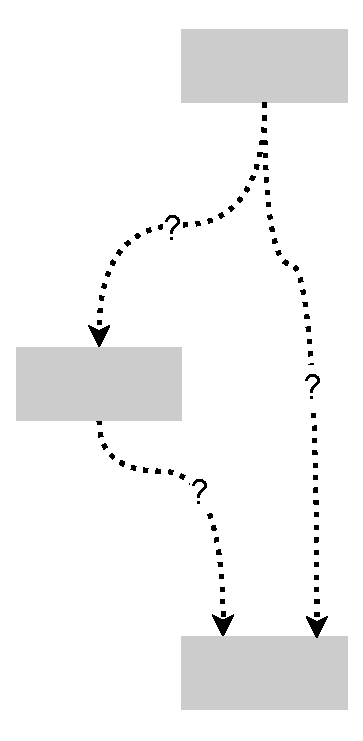
\includegraphics[scale=0.4, center]{graphics/quick/darts_0.drawio.pdf}
\end{figure}
\end{column}
\begin{column}{.3\textwidth}
\end{column}
\begin{column}{.35\textwidth}
\end{column}
\end{columns}
\end{frame}

\begin{frame}{Differentiable Architecture Search}
\vspace{10pt}
\textit{DARTS} \cite{Liu2018} considered as pioneer work
\vfill
\begin{columns}
\begin{column}{.32\textwidth}
\begin{figure}
	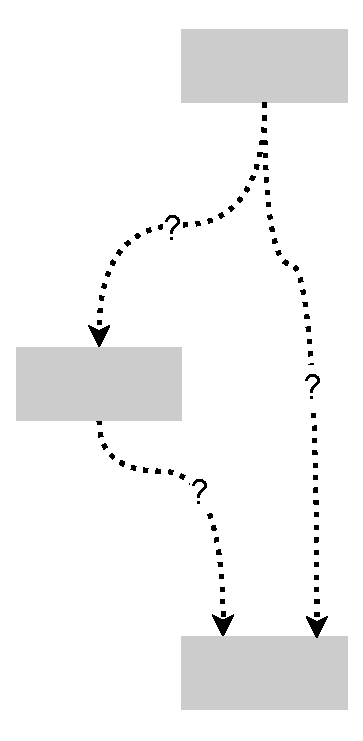
\includegraphics[scale=0.4, center]{graphics/quick/darts_0.drawio.pdf}
\end{figure}
\end{column}
\begin{column}{.68\textwidth}
\begin{figure}
	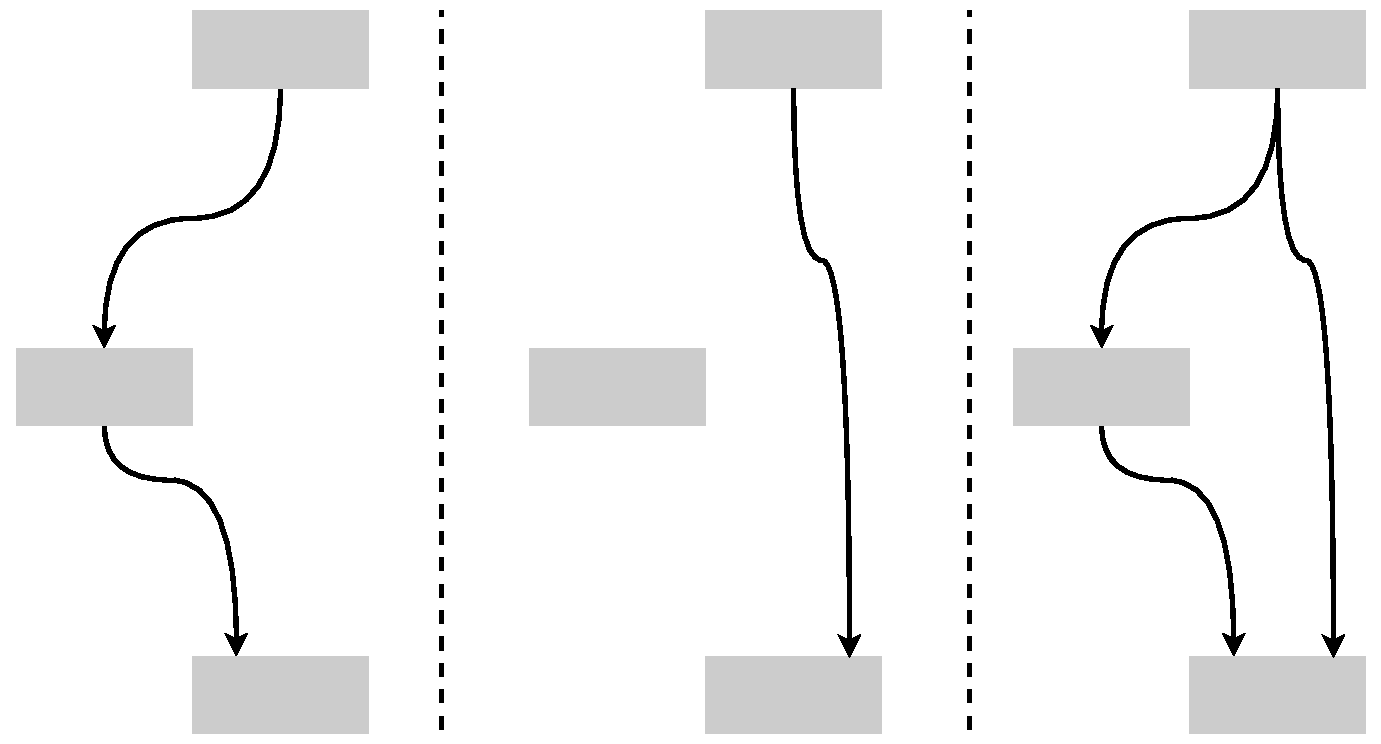
\includegraphics[scale=0.25, left]{graphics/quick/darts_0_candidates.drawio.pdf}
\end{figure}
\end{column}
\end{columns}
\end{frame}

\begin{frame}{Differentiable Architecture Search}
\vspace{10pt}
\textit{DARTS} \cite{Liu2018} considered as pioneer work
\vfill
\begin{columns}
\begin{column}{.35\textwidth}
\begin{figure}
	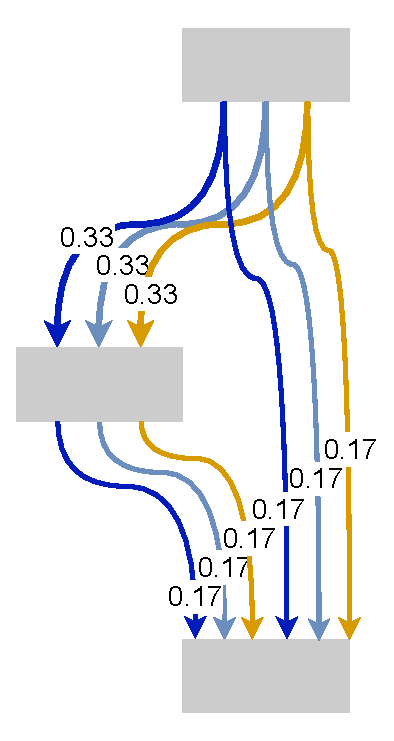
\includegraphics[scale=0.4, center]{graphics/quick/darts_1.drawio.pdf}
\end{figure}
\end{column}
\begin{column}{.3\textwidth}
\end{column}
\begin{column}{.35\textwidth}
\end{column}
\end{columns}
\end{frame}

\begin{frame}{Differentiable Architecture Search}
\vspace{10pt}
\textit{DARTS} \cite{Liu2018} considered as pioneer work
\vfill
\begin{columns}
\begin{column}{.35\textwidth}
\begin{figure}
	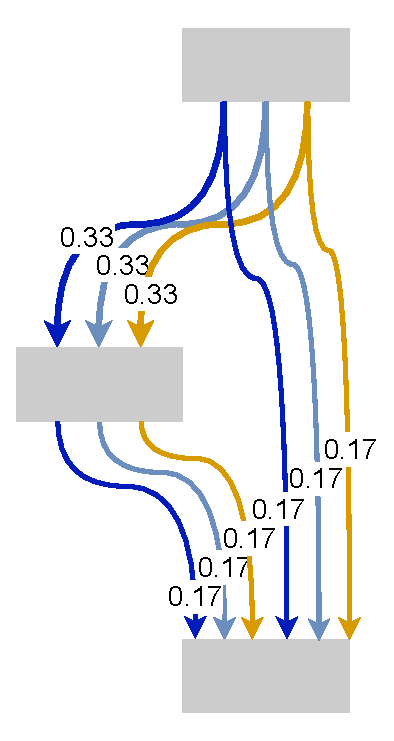
\includegraphics[scale=0.4, center]{graphics/quick/darts_1.drawio.pdf}
	\caption{Training start}
\end{figure}
\end{column}
\begin{column}{.3\textwidth}
\begin{figure}
	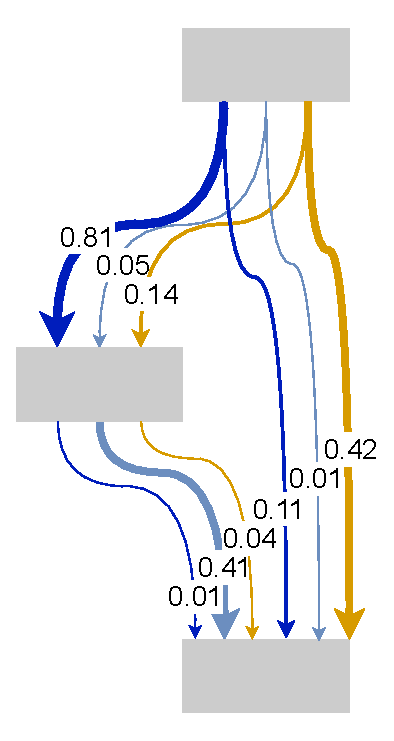
\includegraphics[scale=0.4, center]{graphics/quick/darts_2.drawio.pdf}
	\caption{Training end}
\end{figure}
\end{column}
\begin{column}{.35\textwidth}
\begin{figure}
	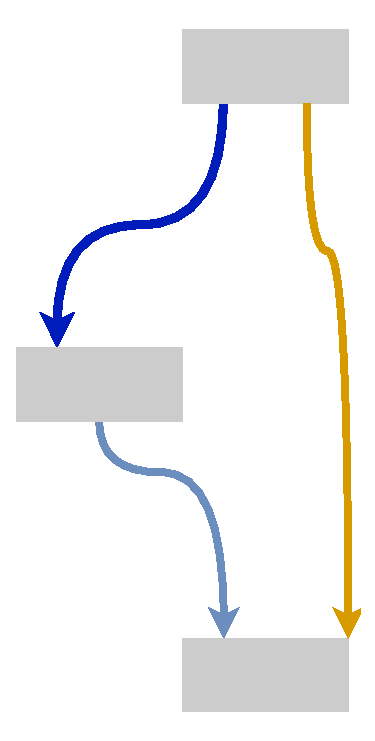
\includegraphics[scale=0.4, center]{graphics/quick/darts_3.drawio.pdf}
	\caption{Obtain best architecture}
\end{figure}
\end{column}
\end{columns}
\end{frame}

\section{DARTS as Surrogate}
\begin{frame}{Search Space}
\vspace{5pt}
\vfill
\begin{columns}
\begin{column}{.96\textwidth}
\begin{figure}
    \begin{center}
    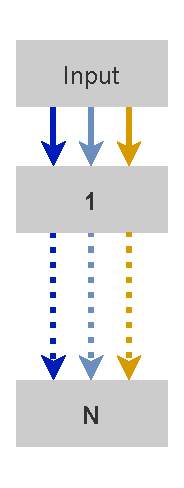
\includegraphics[scale=.85]{graphics/quick/search_space.drawio.pdf}
  \end{center} 
\end{figure}
\end{column}
\begin{column}{.04\textwidth}
\end{column}
\end{columns}
\end{frame}

\begin{frame}{Search Space}
\vspace{14pt}
\vfill
\begin{figure}
    \begin{center}
    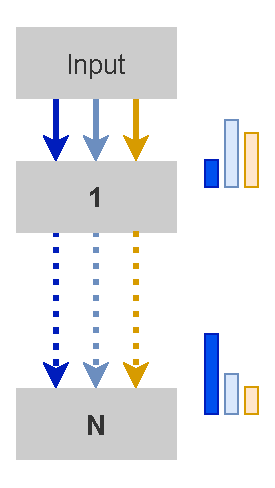
\includegraphics[scale=.8]{graphics/quick/search_space_incl_sampling_prob.drawio.pdf}
  \end{center} 
\end{figure}
\end{frame}

\begin{frame}{DARTS Surrogate}
\vspace{10pt}
\vfill
\begin{figure}
    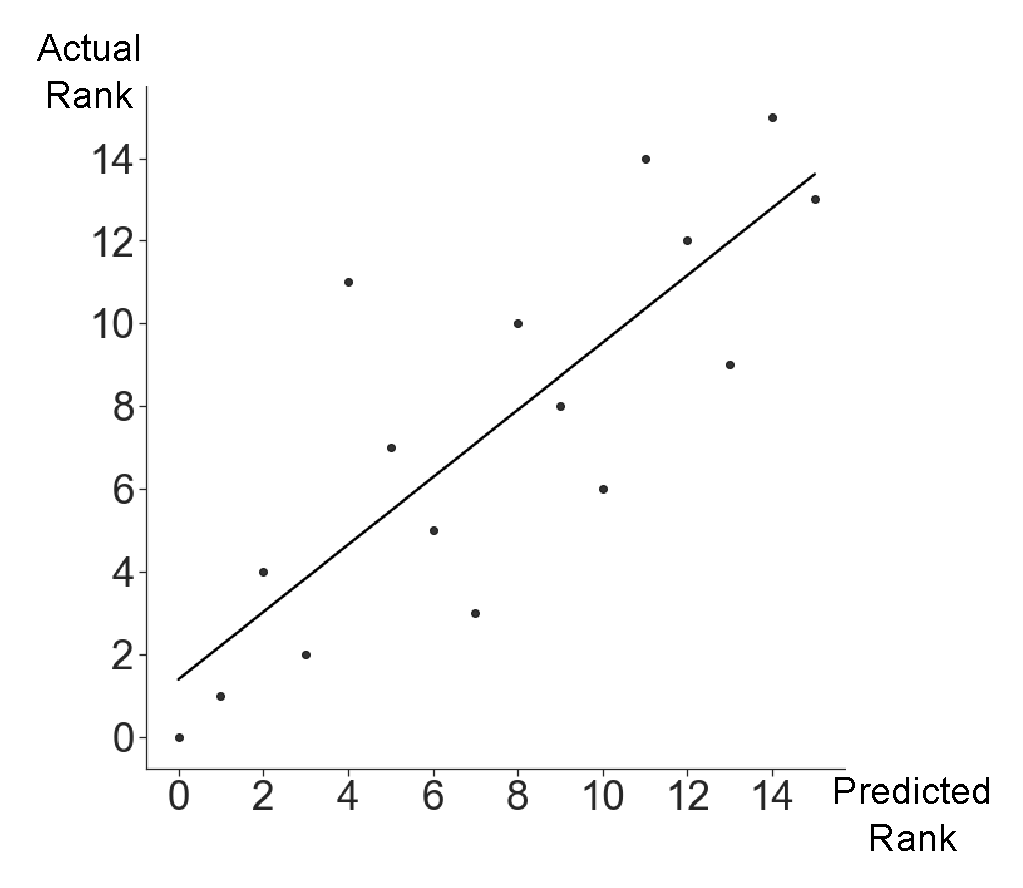
\includegraphics[scale=0.5, center]{graphics/spearman_validation.pdf}
\end{figure}
\end{frame}

\begin{frame}{Architecture Plasticity}
\vspace{10pt}
\vfill
\begin{figure}
    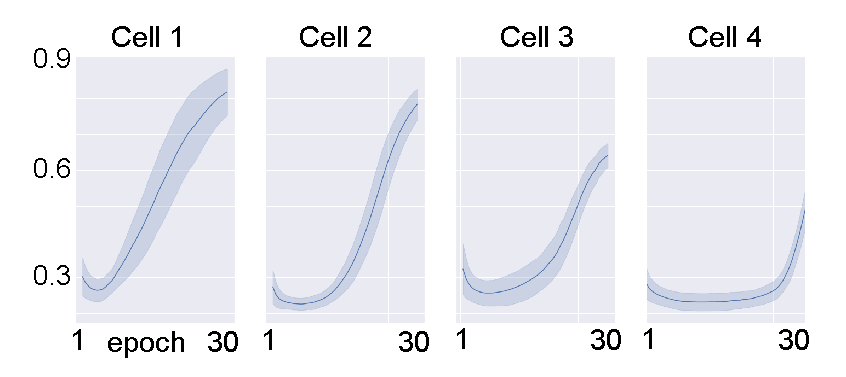
\includegraphics[scale=0.75, center]{graphics/alpha_curves.pdf}
    \caption{Maximum norm of architecture parameter vector per epoch per cell}
\end{figure}
\end{frame}

\section{Beyond Finite Search Spaces}
\begin{frame}{Search Space Extension}
\vspace{10pt}
\vfill
\begin{figure}
    \begin{center}
    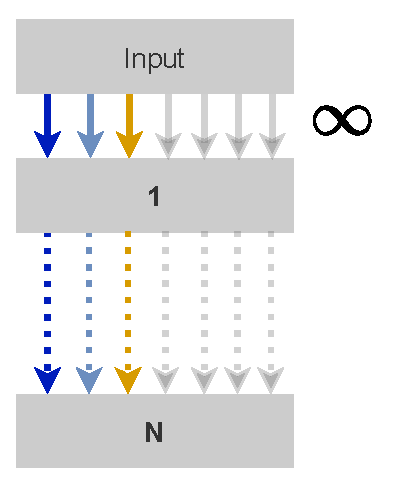
\includegraphics[scale=0.8]{graphics/quick/search_space_extension.drawio.pdf}
    \caption{}
  \end{center} 
\end{figure}
\end{frame}

\begin{frame}{Finite Difference Descent}
\vspace{20pt}
\vfill
\begin{figure}
\begin{center}
\begin{overprint}
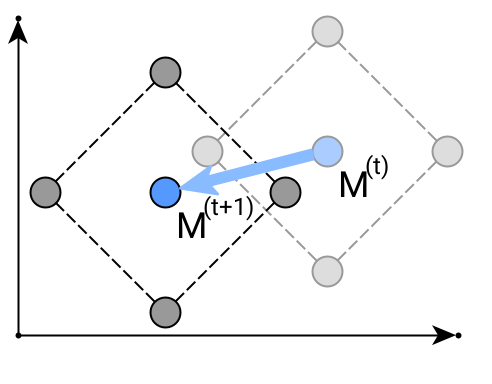
\includegraphics[scale=0.32, center]{graphics/v2_window.png}
\caption{2-dim euclidean search space}
\end{overprint}
\end{center}
\end{figure}
\end{frame}

\begin{frame}{Experiment Results}
\vspace{10pt}
Top $10$ architectures found by Random Search, Bayesian Search and our approach
\vfill
\begin{figure}
    \begin{center}
    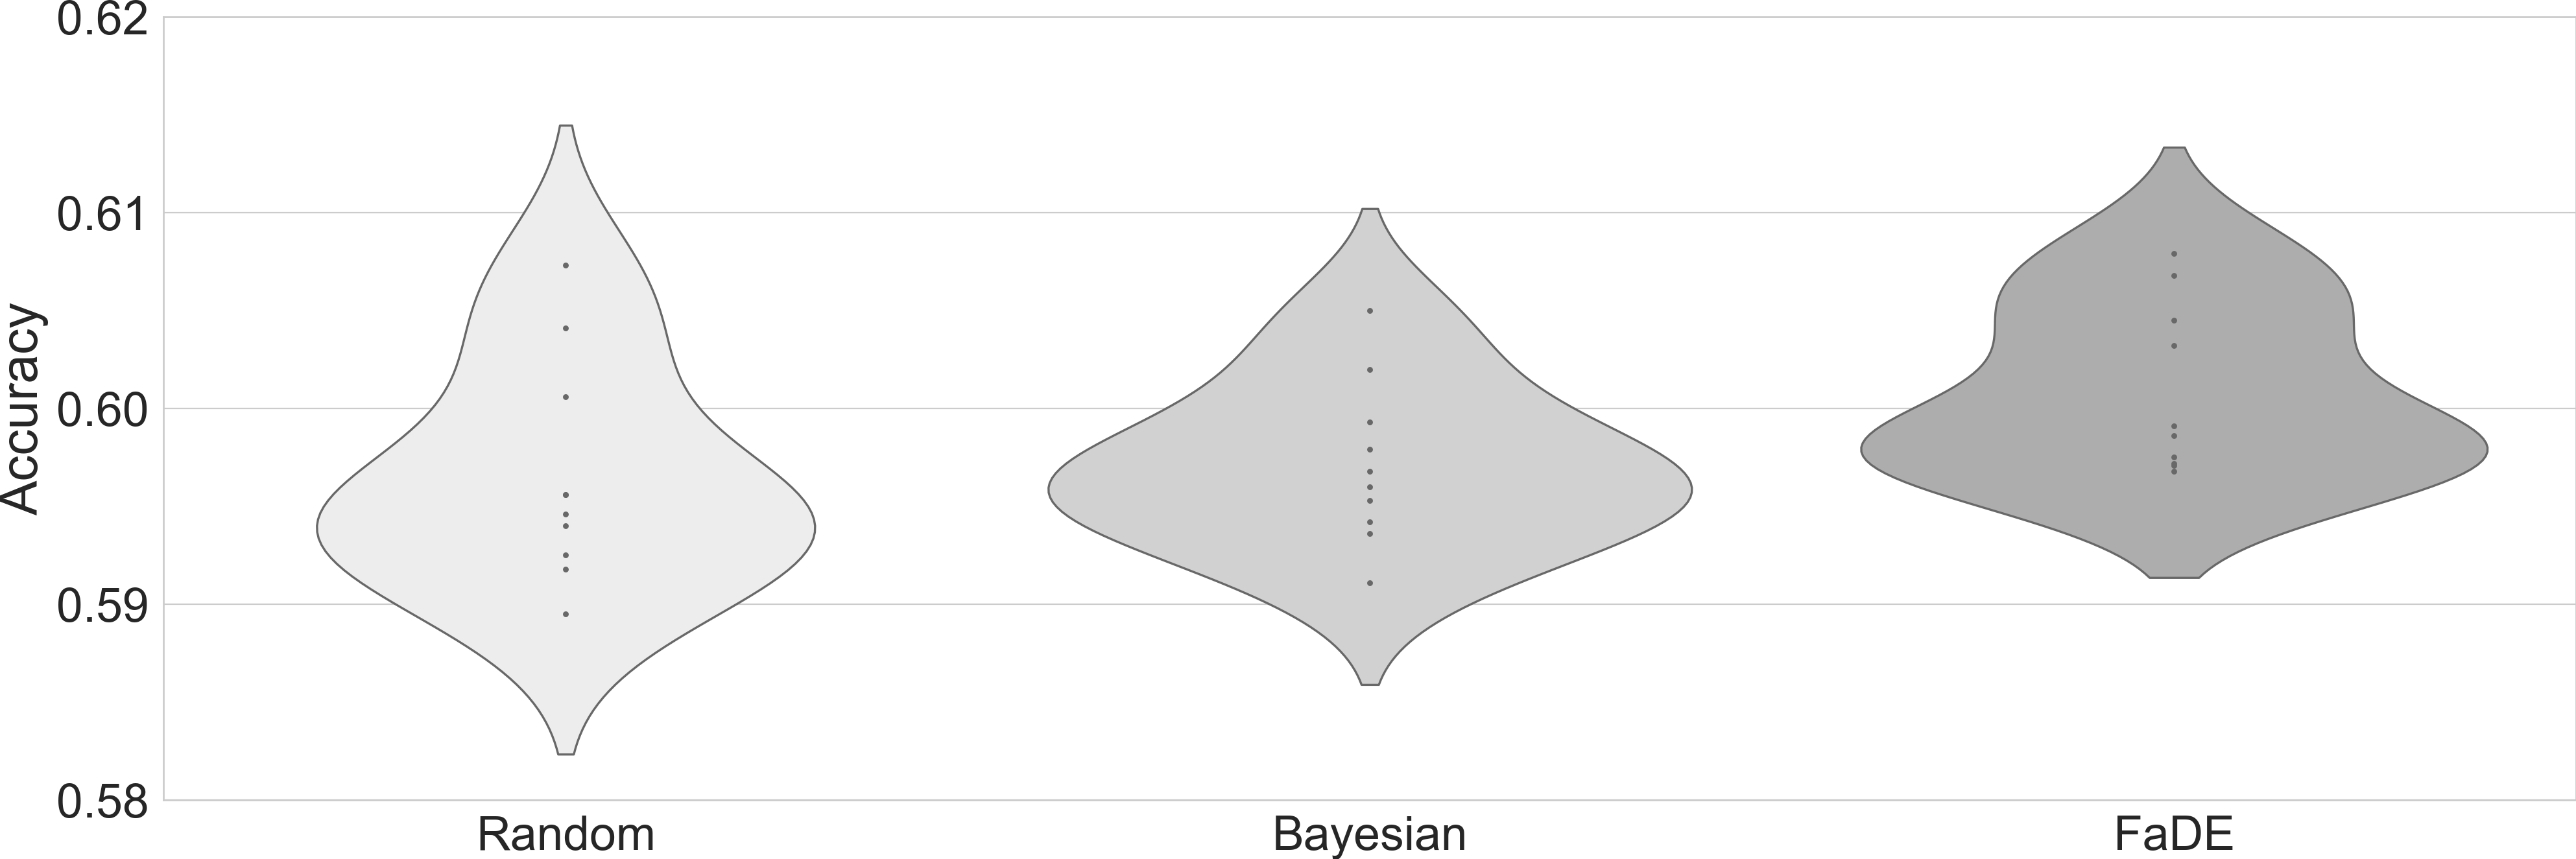
\includegraphics[scale=.22]{graphics/benchmark.png}
    \caption{}
  \end{center} 
\end{figure}
\end{frame}

\begin{frame}{References}
\bibliographystyle{apalike}
\bibliography{bib}
\end{frame}

\end{document}
